\documentclass[]{article}
\usepackage{graphicx}
\usepackage{hyperref}
\usepackage{listings}
\usepackage{xcolor}

\definecolor{gray}{RGB}{245,245,245}
\definecolor{light-gray}{gray}{0.95}
\newcommand{\code}[1]{\colorbox{light-gray}{\texttt{#1}}}

\lstset{
	aboveskip=1ex,
	basicstyle=\ttfamily,
	belowskip=1ex,
	breaklines=true,
	columns=fullflexible,
	framerule=0pt,
	framexrightmargin=0em,
	framexleftmargin=0em,
	numberstyle=\footnotesize\sffamily,
	tabsize=2,
	backgroundcolor=\color{gray}
}
%opening
\title{DECODER MORSE SIGNAL INTO TEXT}
\author{Reza Ali Nirwansyah}



\begin{document}

\maketitle

\begin{abstract}

\end{abstract}

\section{Latar Belakang}

Kode Morse adalah sistem komunikasi yang menggunakan tanda titik dan tanda strip untuk mempresentasikan huruf dan angka. Kode morse dapat digunakan sebagai alternatif sistem pengiriman pesan dengan menggunakan alat komunikasi sederhana yang mana tidak mampu mengirim pesan yang sangat komplek, seperti radio yang hanya dapat mengirimkan sinyal beep, cahaya kilat, suara klakson dan lain sebagainya.

Namun, untuk dapat membaca sinyal kode morse, diperlukan kemampuan untuk mendekode kan pola tanda titik dan strip untuk mendapatkan pesan yang ingin disampaikan. Oleh karena itu, Proyek “DECODER MORSE SIGNAL INTO TEXT” bertujuan untuk melakukan dekode sebuah kode morse dalam bentuk audio morse menjadi teks dengan menggunakan teknik pengolahan sinyal digital.

Dengan adanya sistem decode morse yang otomatis, kita dapat mengubah sinyal audio morse menjadi teks dengan cepat, tepat, dan akurat. Ini dapat digunakan sebagai alat komunikasi rahasia, penyandian pesan rahasia, dan transmisi data dalam situasi yang membutuhkan komunikasi non-verbal.

\section{Cara Kerja}
Berikut ini merupakan cara kerja dari proyek "DECODER MORSE SIGNAL INTO TEXT" yang dijelaskan dalam langkah-langkah berikut.
\begin{itemize}
	\item Perekaman Sinyal Audio : Sinyal audio morse dapat direkam menggunakan perangkat rekaman dalam format .wav yang berisikan pola tanda titik dan tanda strip. Tapi untuk proyek kali ini, menggunakan dataset yang telah disediakan
	
	\item Data Cleaning : Sinyal audio morse yang telah didapatkan kemudian dibersihkan terlebih dahulu. Grafik sinyal yang awalnya mentah kemudian dirapikan sesuai kebutuhan. Dalam kasus ini data akan di filter agar lebih memudahkan dalam mengidentifikasikan mana tanda Titik (dot) atau Strip (Dash)
	
	\item Identifikasi Tanda Titik (dot) dan Tanda Strip (Dash) : Dalam domain waktu. terdapat perbedaan durasi antara Dot dan Dash. sehingga perlu kita analisa untuk mengetahui panjang durasi untuk Dot dan Dash. Selain mengidentifikasi kan panjang durasi dot dan dash. Diperlukan juga analisa untuk mengetahui perbedaan apakah ada tanda spase atau garis miring.
	
	\item Dekode Morse Signal :  Setelah tanda titik dan tanda strip dapat diidentifikasi, pola tersebut diterjemahkan menjadi karakter teks dalam kode Morse. Kamus Morse digunakan untuk melakukan pemetaan antara pola tanda dengan karakter teks yang sesuai.
	
	\item Rekonstruksi Teks : Karakter teks dalam kode morse yang didekode kemudian disusun kembali menjadi kata-kata dan kalimat yang dapat dibaca. Teks yang didekode kemudian ditampilkan sebagai hasil Akhir
\end{itemize}

\section{Pembahasan}
\subsection{Perekaman Audio}
Pada proses perekaman audio. Penulis memanfaatkan data set yang telah disediakan oleh kaggle.com. sehingga penulis tidak melakukan perekaman secara langsung.
% TODO:  required
\begin{center}
	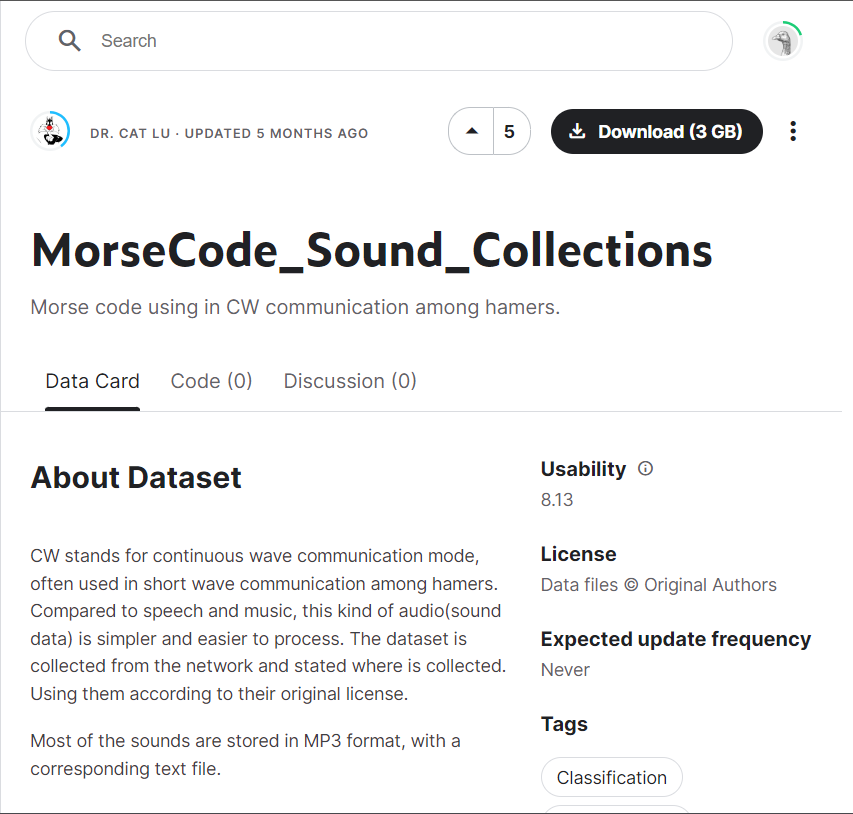
\includegraphics[width=0.7\linewidth]{img/screenshot001}
\end{center}
untuk link dataset nya dapat diakses di link berikut : 
\href{https://www.kaggle.com/datasets/bg4xsd/morse-sound}{Dataset Morse Signal}

\subsection{Data Cleaning}
Setelah data didapatkan, data diolah terlebih dahulu. langkah pertama yang dilakukan adalah melakukan normalisasi terlebih dahulu. dimulai dari perubahan rentang audio sehinga menjadi antara 0 dan 1. kemudian data ini dipresentasikan setiap sampel ke 200. sehingga hasil yang didapatkan seperti ini.
\begin{center}
	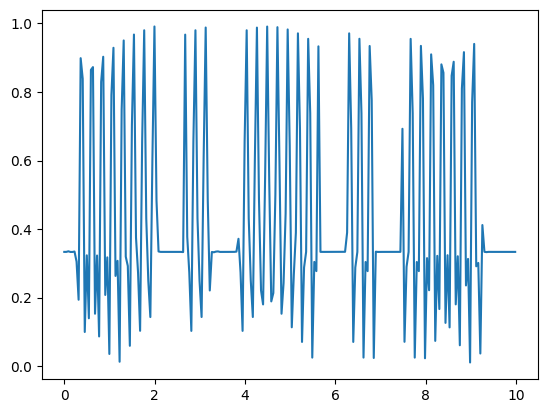
\includegraphics[width=0.7\linewidth]{img/screenshot005}
\end{center}
dari data tersebut terlihat bagian mana yang dash, dan bagian mana yang dot. Tetapi panjang dari suara tidak rata. sehingga proses berikutnya akan sedikit sulit. Sehingga proses berikutnya adalah meratakan sinyal audionya. sehingga jika ada suara, sinyal akan memiliki panjang 1, jika tidak maka 0.
\begin{center}
	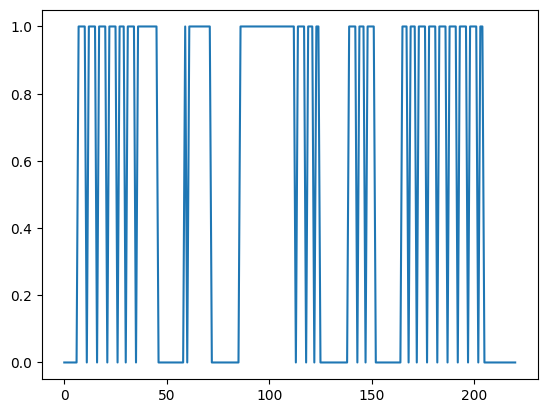
\includegraphics[width=0.7\linewidth]{img/screenshot004}
\end{center}
pada gambar diatas, masih terdapat ketidak rapian. khususnya bagian dot dan dash yang mana masih ada sinyal yang bernilai 0. kita perlu mengubah sinyal itu menjadi bernilai 1. agar bentuk dari dot atau dash sudah mulai terlihat. hal yang dilakukan adalah jika ada sinyal yang bernilai 0, apakah sinyal sebelum dan sesudahnya bernilai 1? jika iya ganti nilai sinyal tersebut menjadi 1, jika tidak biarkan saja. Sehingga hasilnya menjadi seperti ini.
\begin{center}
	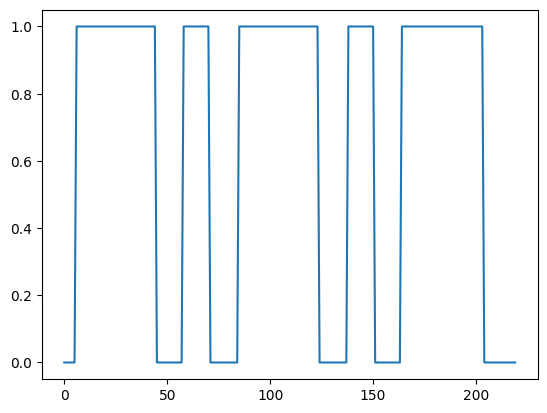
\includegraphics[width=0.7\linewidth]{img/screenshot006}
\end{center}
Setelah melakukan berbagai pengolahan data sehingga menghasilkan data yang demikian. data tersebut kemudian dapat digunakan untuk proses selanjutnya.

\subsection{Identifikasi Tanda Titik (dot) dan Strip (dash)}
Pada tahap ini, data yang dimiliki sudah bersih. sehingga dapat dilakukan proses selanjutnya. 

untuk mengidentifikasi panjang dot dan dash. diperlukan membuat array yang berisi panjang durasi setiap signal. dari proses tersebut didapatkan seperti ini.
\begin{center}
	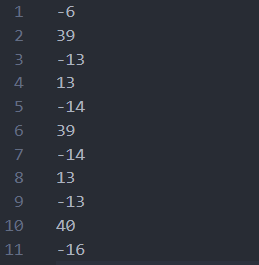
\includegraphics[width=0.7\linewidth]{img/screenshot007}
\end{center}
angka angka tersebut menunjukkan durasi masing masing signal. angka yang negatif menunjukkan durasi sinyal yang bernilai 0. dan angka yang positif menunjukkan durasi sinyal yang bernilai 1.

Pada visual yang telah kita lihat, kombinasi dot dan dash nya  adalah -.-.- (dash dot dash dot dash). dan pada data durasi, panjang durasi dari signal yang bernilai 1 adalah [39, 13, 39, 13, 40]. Jadi dapat disimpulkan bahwa panjang untuk dot adalah kurang dari 20. dan panjang dari dash adalah lebih dari 20. Mengapa menggunakan rentang daripada angka yang pasti. hal itu dilakukan untuk mencegah kesalahan karena panjang dari sebuah signal tidak memiliki angka yang tetap.

selain mengidentifikasi dosh dan dat. diperlukan juga untuk mengidentifikasi spasi (' ') dan garis miring ('/'). dari data yang didapat panjang dari antar simbol adalah kurang dari 20. panjang untuk spasi adalah kurang dari 50. dan jarak untuk garis miring adalah lebih dari 150

\begin{center}
	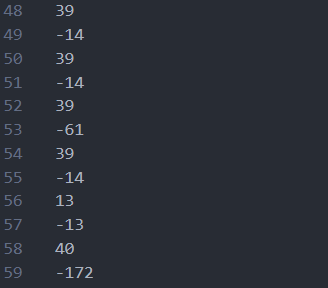
\includegraphics[width=0.7\linewidth]{img/screenshot008}
\end{center}

\subsection{Dekode Morse Signal}
Setelah melakukan identifikasi panjang dot dan dash. Yang selanjutnya dilakukan adalah mengubah kumpulan array durasi tersebut menjadi kumpulan kode morse. Cara yang dilakukan adalah membuat perluangan sepanjang array durasi. kemudian buat array baru. jika nilai nya positif itu adalah signal, jika negatif, itu adalah bagian yang hening.

\begin{lstlisting}
morse_code = ""

for morse in data3:
	if morse > 0:
		if morse < 20:
			morse_code += '.'
		elif morse > 20:
			morse_code += '-'
	elif morse < 0:
		if abs(morse) > 150:
			morse_code += '/'
		elif abs(morse) > 50:
			morse_code += ' '
\end{lstlisting}

sehingga hasil yang didapatkan adalah

\begin{lstlisting}
-.-.-/- .... .. .../. -... --- --- -.-/.. .../..-. --- .-./- .... ./..- ... ./--- ..-./.- -. -.-- --- -. ./.- -. -.-- .-- .... . .-. ./.- -/-. ---/-.-. --- ... -/.- -. -../.-- .. - ..../.- .-.. -- --- ... -/-. ---/.-. . ... - .-. .. -.-. - .. --- -. .../.-- .... .- - ... --- . ...- . .-. .-.-.-/-.-- --- ..-/-- .- -.--/-.-. --- .--. -.--/.. - --..--/--. .. ...- ./.. -/.- .-- .- -.--/--- .-./.-. . -....- ..- ... ./.. -/..- -. -.. . .-./- .... ./- . .-. -- .../--- ..-./- .... ./.--. .-. --- .--- . -.-. -/--. ..- - . -. -... . .-. --./.-.. .. -.-. . -. ... ./.. -. -.-. .-.. ..- -.. . -../.-- .. - ..../- .... .. .../. -... --- --- -.-/--- .-./--- -. .-.. .. -. ./.- -/.-- .-- .-- .-.-.- --. ..- - . -. -... . .-. --. .-.-.- --- .-. --./-...- -.. . .- - ..../--- ..-./.-/... .--. .- -.-. . -- .- -./-... -.--/.-- .- .-.. - . .-./-- .-.-.-/-- .. .-.. .-.. . .-. --..--/.--- .-. .-.-.-/-...- --- .-.. -../-.. --- -. . --. .- .-../.-- .- .../-.. -.-- .. -. --. .-.-.-/- .... . -.--/.... .- -../.- .-.. .-../-.- -. --- .-- -./.. -/.-- .- .../-.-. --- -- .. -. --. --..--/.- -. -../- .... . -.--/.-- .- - -.-. .... . -../.. -/-.-. --- -- . -....- -....- .... .. .../.... .- --. --. .- .-. -../.-- .. ..-. . --..--/.... .. .../-.. .- ..- --. .... - . .-. --..--/.- -. -../-. --- .--/.... .. .../--. .-. .- -. -.. ... --- -. --..--/.... --- -- ./--- -./. -- . .-. --. . -. -.-. -.--/.-.. . .- ...- ./..-. .-. --- --/- .... ./.--. .-. . -....- .- ... - .-. --- -. .- ..- - .. -.-. .../.- -.-. .- -.. . -- -.-- .-.-.-/--- .-.. -../-.. --- -. . --. .- .-../-.-
\end{lstlisting}

\subsection{Rekonstruksi Text}

setelah data morse sudah didapatkan. kemudian di decode menjadi text yang bisa kita baca. untuk diperlukan sebuah dictionary dari python yang berisikan terjemahan kode morse nya. berikutnya  memisahkan kode morse setiap ada tanda strip untuk memisahkan antar kata. dan di dalam kata dipisahkan setiap ada spasi untuk memisahkan setiap huruf. sehingga kode yang digunakan adalah.
\begin{lstlisting}
data_morse = {
	'.-': 'A', '-...': 'B', '-.-.': 'C', '-..': 'D', '.': 'E',
	'..-.': 'F', '--.': 'G', '....': 'H', '..': 'I', '.---': 'J',
	'-.-': 'K', '.-..': 'L', '--': 'M', '-.': 'N', '---': 'O',
	'.--.': 'P', '--.-': 'Q', '.-.': 'R', '...': 'S', '-': 'T',
	'..-': 'U', '...-': 'V', '.--': 'W', '-..-': 'X', '-.--': 'Y',
	'--..': 'Z', '.----': '1', '..---': '2', '...--': '3', '....-': '4',
	'.....': '5', '-....': '6', '--...': '7', '---..': '8', '----.': '9',
	'-----': '0', '--..--': ',', '.-.-.-': '.', '..--..': '?',
	'-..-.': '/', '-....-': '-', '-.--.': '(', '-.--.-': ')'
}

decode_text = ""

words = morse_code.split('/')
for word in words:
	character = word.split(' ')
	decode_word = ''
		for char in character:
			if char in data_morse:
			decode_word += data_morse[char]
	decode_text += decode_word + ' '

print(decode_text)
\end{lstlisting}
dan hasil dari decode morse menjadi text yang dibaca adalah

\begin{lstlisting}
THIS EBOOK IS FOR THE USE OF ANYONE ANYWHERE AT NO COST AND WITH ALMOST NO RESTRICTIONS WHATSOEVER. YOU MAY COPY IT, GIVE IT AWAY OR RE-USE IT UNDER THE TERMS OF THE PROJECT GUTENBERG LICENSE INCLUDED WITH THIS EBOOK OR ONLINE AT WWW.GUTENBERG.ORG DEATH OF A SPACEMAN BY WALTER M. MILLER, JR. OLD DONEGAL WAS DYING. THEY HAD ALL KNOWN IT WAS COMING, AND THEY WATCHED IT COME--HIS HAGGARD WIFE, HIS DAUGHTER, AND NOW HIS GRANDSON, HOME ON EMERGENCY LEAVE FROM THE PRE-ASTRONAUTICS ACADEMY. OLD DONEGAL K
\end{lstlisting}

\section{Kesimpulan}
Setelah melakukan proses pengolahan sinyal digita. dapat disimpulkan bahwa untuk melakukan pengolahan sinyal digital tahap tahap yang umum dilakukan adalah filtering data atau cleaning data. intinya data harus  dipersiapkan dulu sesuai dengan kebutuhan sesuai dengan kebutuhan proses yang diperlukan. kemudian tahap berikutnya adalah proses. tahap ini dilakukan berbagai cara seperi compare, mengubah sinyal, dan lain sebagainya.
\end{document}
